
%do not modify
%
%
%
%

\documentclass{report}
\pdfinfo{
    /Author (Eyob Ghebreiesus)
   /Title  (Project HurriSat Final)
   /CreationDate (D:20220215190000)
   /ModDate (\date{today})
   /Subject (Spacecraft Design)
   /Keywords (Spacecraft, HurriSat, Aerospace)
}
\usepackage{placeins}
\usepackage{multirow}
\usepackage{comment}
\usepackage[x11names]{xcolor}
\definecolor{navyblue}{HTML}{002147}
\hypersetup{%
   colorlinks   = true, %Colours links instead of ugly boxes
   urlcolor     = black, %Colour for external hyperlinks
%   linkcolor    = blue, %Colour of internal links
%   citecolor   = red %Colour of citations
}
%%do not modify
\includegraphics[scale=.5]{cover.png}
\newcommand{\HRule}{\rule{\linewidth}{0.4mm}}
\usepackage{wrapfig}
\usepackage{lmodern}
% \usepackage{framed}
\usepackage{graphicx}
\usepackage[export]{adjustbox}
% \usepackage[style=ieee]{biblatex}
% \addbibresource{bibtex.bib}
\usepackage[backend=biber]{biblatex}
\addbibresource{bibtex.bib}
\usepackage{tabularx}
\usepackage{indentfirst}
\usetikzlibrary{shapes, arrows}
\begin{document}
\pagenumbering{roman}
\pagenumbering{gobble}
\setlogo{Logo.png}
\setyear{MMAE-412, 2022}
\begin{center}
\textbf{\color{white}TOP SECRET}\\[.2in]
%\vspace{0.25mm} \\
%\textbf{\color{black}{MMAE-412 SPACECRAFT DESIGN}}\\
% \large\textbf{\href{https://github.com/eyobghiday/project-hurrisat}{Project HurriSat}}\\[.7in]
%\textbf{\small\href{https://github.com/eyobghiday/project-hurrisat}{PROJECT HURRISAT}}
\Large\textsc{\href{https://github.com/eyobghiday/project-hurrisat}{PROJECT HURRISAT}}
\HRule
\vspace{2.2cm}
\end{center}
\begin{figure}[h]
\centering
\includegraphics[width=9cm]{Images/iit_logo.png}\\[.3in]
%\HRule
% \caption*{\small{$^1$Eyob Ghebreiesus}}
\end{figure}
\begin{center}
\begin{center}
  \large{ILLINOIS INSTITUTE OF TECHNOLOGY}\\
  \small{ARMOUR COLLEGE OF ENGINEERING}\\
    \small{SPACECRAFT DESIGN REPORT}\\  
    THE NASA CSLI INITIATIVE\\\\[.5in]
\end{center}
\begin{center}
\textit{\href{https://github.com/eyobghiday/project-hurrisat}{ Project Hurrisat}}\\
\textit{May $4^{th}$, 2022}
\end{center}
\end{center}

\newpage
\begin{center}
\small\textsc{\href{https://github.com/eyobghiday/project-hurrisat}{PROJECT HURRISAT }}\noindent\rule{\textwidth}{0.4pt}
\vspace{.5in}\\
\large Team Structure\\[.1in]
% \end{center}
% \begin{left}
\small{$^1$}\href{mailto:eghebreiesus@hawk.iit.edu}{Eyob Ghebreiesus}. \small{$^2$}\href{mailto:jmcmahon2@hawk.iit.edu}{Jake McMahon}, \small{$^3$}\href{mailto:kbachiyski@hawk.iit.edu}{Kiril Bachiyski}, \small{$^4$}\href{mailto:lpalmatier@hawk.iit.edu}{Liam Palmatier}, \small{$^5$}\href{mailto:tassefa@hawk.iit.edu}{Tewodros Assefa}
\vspace{.2in}\\
\small{$^1$ M.S Aerospace Engineering. Project Manager, Systems engineer for Mission analysis and operations \\
$^2$ B.Sc Aerospace Engineering. Project Requirements, Constraints, and Risk Assessments    \\
$^3$ B.S. Aerospace Engineering. Payload delivery design and Communication Architecture\\
$^4$ M.S. Aerospace Engineering. Power design, Thermal design and Shielding \\
$^5$ M.S. Aerospace. Structures, Propulsion and Thrusters design}\\[1in]
% \end{left}
\end{center}
Homepage: \textit{\href{https://github.com/eyobghiday/project-hurrisat}{Project HurriSat}} \\
Contact: \href{mailto:eghebreiesus@hawk.iit.edu}{ehgbereiesus@hawk.iit.edu}\\
Published on \textit{May $4^{th}$, 2022}\\[.2in]
Copyright © 2022\\
All rights reserved. This Lab report or any portion thereof may not be reproduced or used in any manner whatsoever without the express written permission of the publisher except for the use of referencing for educational purposes.\\
The above copyright notice and this permission notice shall be included in all copies or substantial portions of the document.\\[.2in]
Produced via LaTeX, Inc U.S.A.\\
MIT License for the GitHub Project, 2022\\
\href{https://github.com/eyobghiday/project-hurrisat}{\textit{github.com/eyobghiday/project-hurrisat}}\\
\begin{center}
\href{https://www.iit.edu/mmae}{Department of Mechanical, Materials and Aerospace Engineering}\\
\href{https://www.iit.edu}{ILLINOIS INSTITUTE OF TECHNOLOGY}\\
\end{center}

\newpage
\hypersetup{hidelinks}
% 
\pagestyle{fancy}
\fancyhf{}
\fancyhead[RE,LO]{\includegraphics[height=\logoheight, keepaspectratio, align=c]{\logo}}
\fancyhead[LE,RO]{\href{https://github.com/eyobghiday/project-hurrisat}{Project Hurrisat}}
% \fancyfoot[CE,CO]{\leftmark}
\fancyfoot[CE,CO]{\thepage}
\renewcommand{\headrulewidth}{.8pt}
\renewcommand{\footrulewidth}{.8pt}
% 
\begingroup
\hypersetup{linkcolor=black}
\tableofcontents
\newpage
\pagenumbering{arabic}
\section{Introduction}\label{s:es}
    \subsection{Mission Statement}
The mission of this project is to propose a Low Earth Orbit, 6U sized Cubesat to monitor and track down hurricanes across the South-Atlantic U.S. Region. This Cubesat should be able to measure small to big scale hurricanes across the required region with greater accuracy. It should also be able to record the size of a hurricane, speed, impact area,  changes in temperature, pressure, and other details successfully. By doing so, it has to communicate and transmit data back and forth between local stations effectively. Furthermore, it will ensure the collected data is processed and used as per the contract agreement with the NASA and its interested parties effectively.
\subsection{Mission Relevance to NASA}
HurriSat's mission is in accordance with the first objective of NASA's Strategic plan  \cite{NASA2018} listed in sections 1.1, 1.2, and 3. It's main goal is to study the causes & effects of severe space weather events, and prevent potential damage. Additional criteria in addressing the National Challenges and Catalyze economic growth for space sustainability. Climate change greatly increases the severity and frequency of hurricanes and other extreme weather. This has led to a significant need for fast and accurate weather data in order to prevent and reduce catastrophic damages. This feasibility report ensures HurriSat meets the requirements and objective outlined by NASA in the CSLI \cite{CLSI} initiative.

This document provides a refined look at the mission analysis and concept of operations for HurriSat. The mission goals and objectives are laid out, and the analysis plan is discussed in detail. The conceptual design and analysis takes a scientific approach towards the concept of operations. Here the criteria from the NASA CLSI missions are analyzed and turned into either requirements or constraints. Alternate plans for the mission are also discussed in later section. Furthermore, a brief evaluation is conducted for each subsystem and its purpose in the mission according to the project plan.

\subsection{Background in Hurricanes}
    \begin{wraptable}{r}{0.5\textwidth}
    \centering
    \begin{tabular}{ccr}
    \rowcolor{gray!50}{Category & Speed (mph) & Severity}\\
    \cellcolor{red!20} 1  & { $74-95$} & {\small Minimal damage}\\
    \cellcolor{red!40} 2  & { $96-110$} & {\small Considerable damage}\\
    \cellcolor{red!60} 3 & { $111-129$} & {\small Extreme damage}\\
    \cellcolor{red!80} 4 & { $130-156$} & {\small Devastating}\\
    \cellcolor{red} 5 & { $>156$} & {\small Catastrophic}\\
    \end{tabular}
    \caption{\small Hurricane Severity}
    \label{Tab:hss}
\end{wraptable} 
    Hurricanes are among the most destructive weather phenomena that are caused by strong winds and surge effects. They can be fatal, and usually cause destruction of infrastructures. In 2012, Hurricane Sandy led to about $\$65$ billion damage in the northeastern coastal region of the USA and in the Ontario Province of Canada \cite{Cui2016}. The severity of the consequences, associates with hurricane activity, has motivated several investigations, attempting to forecast hurricane activity in both near and distant future. Hurricanes are primarily classified based on their speed as seen in Table \ref{Tab:hss}, with Category 5 being the most severe. This serves as one of the many reasons that led us bring forward project HurriSat to NASA and its affiliates. Therefore, HurriSat's sole mission will be dedicated to tracking, monitoring and possibly avoiding fatal devastation caused by hurricanes. Additionally, HurriSat will be equipped with high-tech cameras and faster processor to provide accurate weather data with little to zero maintenance cost.

\subsection{Stakeholders and Customers} The stake holders partly consist of with an interest with the enterprise  of NASA and its affiliates. They are divided into two main categories, Primary and Secondary stakeholders as listed in Table \ref{Tab:st}. Those stakeholders may include those listed but not limited to:
\begin{atn}[H]{Stakeholders}{tab:sh}{l l @{\hskip 25pt} r r}
    \textcolor{black}{Primary Stakeholders} & Secondary Stakeholders \\
    NASA & Department of Education\\
    National Weather Service & National Environmental Satellit\\
    Federal Emergency Management Agency &  NOAA \\
    Department of Defense & Others: Public Safety, Health and Red cross \\
\label{Tab:sh}
\end{atn}   

\section{Mission Exploration}\label{s:ms}
    The mission of this project is to propose a Low Earth Orbit 6U sized Cubesat in order to track down the hurricanes across the South-Atlantic U.S. Region. The primary target coverage area is about 110,000 square miles across the South East-cost. This Cubesat should be able to track small to big size hurricanes across the given region. This is mainly achieved using high-tech dual cameras. It will try to collect the speed, impact area,  changes in temperature, pressure, and air composition of earth’s atmosphere for a given radius in miles. By doing so, it has to communicate and transmit data back and forth between local stations effectively. Furthermore, we must ensure the recorded data is shared with the outlined stakeholders and interested parties effectively. 
\subsection{Mission Objectives }
Our primary and secondary mission objectives are as follows.
\subsubsection{Primary  Objectives}
\begin{itemize}[noitemsep]
  \item Data recording (Wind speed, hurricane trajectory, impact radius) and analysis.
  \item Transmission of data to and from ground station up to 10 external entities.
  \item Cubesat autonomous tasking if necessary, and warning category level for immediate action.
  \item Navigation and monitoring hurricane impacted areas. Assessing damage on infrastructures to a certain degree.
  \item Updating locations using on board GPS or grounds station.
\end{itemize}
\subsubsection{Secondary Objectives }
\begin{itemize}[noitemsep]
  \item Recording relevant data (Temperature, Pressure, Humidity) for scientific study  .
  \item Maintaining communication with weather stations every $15-20m$ minutes.
  \item Guidance and Navigation of hurricane free zones.
  \item Remote sensing capabilities and effective communication with nearby satellites to avoid debris and collision course. 
\end{itemize}

\subsection{Requirements}
\subsubsection{Functional Requirements}
\begin{itemize}[noitemsep]
  \item 
  Cubesat shall coverage a minimum of 2400x1300 square km (110,00 square miles) ground area for hurricane monitoring.
 \item 
 Cubesat shall provide 2 visible spectrum images with up to 10m/pixel or lower for narrow field, and upto 100m-200m/pixel or max for a wide range of hurricane resolution.
\item
Spacecraft shall provide temperature, relative speed, & atmospheric readings of hurricane (use infrared cam).  
\item
Must able to transmit to ground station without having to rotate the spacecraft.
  \item Responsiveness: Transmitting 3 24-bit color depth images to the ground station over a single pass spanning 15 minutes.
\end{itemize}
\subsubsection{Operational Requirements}
\begin{itemize}[noitemsep]
  \item Duration: Will have a mission life of at least 15-20 years
  \item Availability: 12-hour maximum outage provided space weather conditions.
  \item Reliable: Provided no external and uncontrolled space phenomenon.
  \item Communication: Updates every 15-20 min per by pass.
  \item Data content: Images, location, relative speed, hurricane radius, impact area, atmospheric data, weather prediction and forecast.
  \end{itemize}\\
\subsubsection{Subsystem Requirements and Constraints}
After going over the mission requirements, the subsystem components are inspected and checked to see if they can meet the mission purpose.  Figure \ref{fig:ssreq} goes over all our subsystem designs and lists whether that specific component's requirement and constraint. This in return shapes our design and component selection process. \\
\FloatBarrier
\begin{figure}[hbt!]
    \centering
    \includegraphics[width=\textwidth, frame]{Images/ss_req.png}
    \caption{Subsystem Requirements and Constraints}
    \label{fig:ssreq}
\end{figure} \\

\subsection{Analysis and Trade Studies}
To ensure our project results in designing an effective and efficient cubesat, we have made a project plan to provide the best out put parameters in Figure \ref{fig:manplan}. After initial mission definition the project is closely followed by trade studies. Numerous data for previous successful missions were collected firsthand. The Japanese XI \cite{EoPortal2002} cubesat, the Freja \cite{Freja} cubesat, and the Firesat from the Space mission and design \cite{Larson1999} reference were used as a basis. Those projects solely match our functionality requirements for a 1U-12U cubesat. Figure \ref{fig:graph}(a) is the volume (density) of cubesats at various altitude. It shows 6U-sats are commonly used for a wide range of altitude. If HurriSat is to be equipped with a faster imaging cameras, and max transfer (bandwidth) frequency as shown in Figure \ref{fig:graph}(b), it will require high throughput (red-accent) power. The tradeoff is an increase in mass size as shown in Figure \ref{fig:graph}(c). The inclination distribution of cubesats is graphed in Figure \ref{fig:graph}(d) in order to provide some insight on satellite footprint with mass and altitude. 
Once we select the performance metrics, we use STK \cite{AGISolutions2021} software analysis to test the values in the simulation. After reading the feedback from the simulation; if the findings are feasible, we proceed to component design phase. If not, we go back to refine our mission definition and operational requirements. This is an agile project managing system where we select the performance parameters and perceive the coverage, operation orbit and bypass simultaneously to decide the best fit. This allows us to be flexible with the little time provided.

\tikzstyle{decision} = [diamond, fill=gray!50, text badly centered, node distance=3cm, inner sep=0pt]
\tikzstyle{block} = [rectangle, fill=red!37, text centered, rounded corners, minimum height=4em]
\tikzstyle{line} = [draw, -{Latex[width=5pt,length=7pt]}]
\tikzstyle{cloud} = [ellipse, fill=iitred, node distance=3cm, minimum height=2em]
\vspace{0.5cm}
\begin{figure}[H]
\caption{Mission Analysis}
    \centering
    \begin{tikzpicture}[node distance = 2cm, auto, text=black, inner sep=5pt, align=center]
        % Place nodes
        \node [block] (design) {Mission Definition};
        \node [block, right of = design, node distance = 3.5cm] (manufacturing) {Trade Study};
        \node [block, right of= manufacturing, node distance = 3.5cm] (assembly) {STK Analysis};
        \node [block, right of= assembly, node distance = 3.5cm] (testing) {Testing};
        \node [block, below of= assembly, node distance = 2cm] (feedback) {Feedback};
        \node [block, right of= testing, node distance = 3.5cm] (final) {CubeSat};
        
        % Draw edges
        \path [line] (design) -- (manufacturing);
        \path [line] (manufacturing) -- (assembly);
        \path [line] (assembly) -- (testing);
        \path [line] (testing) |- (feedback);
        \path [line] (feedback) -| (design);
        \path [line] (testing) -- (final);
    \end{tikzpicture}
    \label{fig:manplan}
\end{figure}
\begin{figure}[h!]
  \centering
  \subfloat[Cubesat size scatter vs altitude.]{\includegraphics[width=0.5\textwidth,scale=0.7]{Images/unit.pdf}\label{fig:unit}}
  \hfill
  \subfloat[Downlink Freq over power per unit size.]{\includegraphics[width=0.5\textwidth,scale=0.7]{Images/down.pdf}\label{fig:down}}
 \par\medskip
%   \hfill% or \hspace{5mm} or \hspace{0.3\textwidth}
  \subfloat[Power Loading]{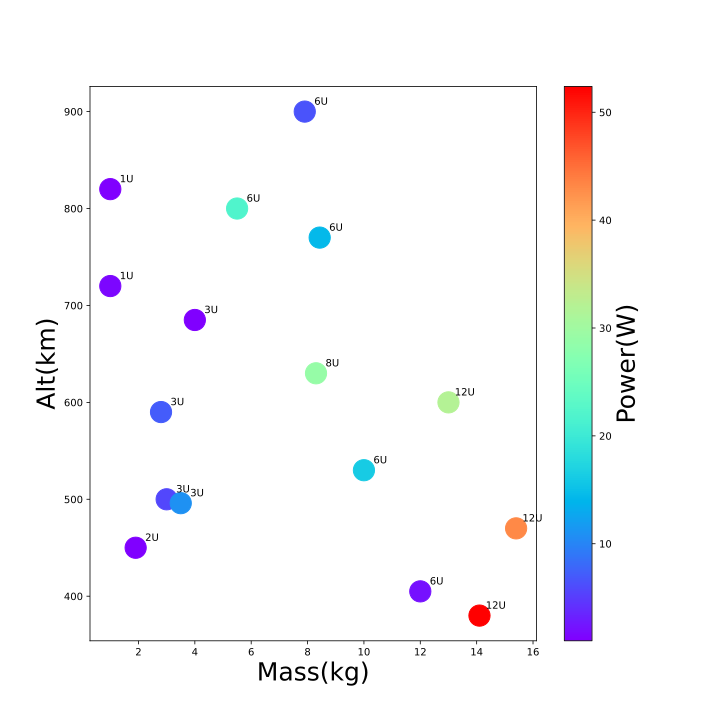
\includegraphics[width=0.5\textwidth,scale=0.9]{Images/power.pdf}\label{fig:power}}
  \hfill
  \subfloat[Inclination]{\includegraphics[width=0.5\textwidth,scale=0.9]{Images/Alpha.pdf}\label{fig:alpha}}
  \caption{Trade Studies}
  \label{fig:graph}
\end{figure}\\

\subsection {Risk Assessment}
Risk assessment assures the stakeholders whether our cubesat  is on track to be hazard free, secure, safe, and scientifically feasible. It is impossible to avoid risks completely. Thus, the team has provided a risk assessment definition in Table \ref{Tab:rd}. Those definitions are basic guideline to help assessing the risks and provide some mitigation mechanisms. They are divided in to two sections: probability and severity. Probability is the likelihood of risk to occur, while severity is the effect of the risk. To determine the risk assessments a color grading scale is provided in Table \ref{Tab:rcg}. Bright red is a high probability  and extremely severe. This risk will definitely hinder all types of operation and may even lead to complete failure of the mission. Green on the other hand is quite the opposite.\\

\begin{table}[hb!]
\centering
\caption{Risk Definitions}
\label{Tab:rd}
\begin{tabular}{ l l }
    \rowcolor{gray!50}{Risk Probability & Description}\\ \hline
    Frequent & Consistent threat to mission. Requires deliberate and active planning. \\
    Occasional& May occur a couple-three times.\\
    Improbable & Highly unlikely to occur.\\[.1in]
    \rowcolor{gray!50}{Risk Severity & Description}\\ \hline
    Catastrophic   & Would cause complete mission failure. It's a no-go situation.\\
    Major         & Would cause significant complication to mission.\\
    Minor         & Would causes a minor  hindrance to mission.\\
    Negligible    & Minimal effect on mission.        
\end{tabular}
\end{table}
\vspace{1.5cm}
\begin{table}[hbt!]
\caption{Risk Color-grading}
\label{Tab:rcg}
\centering
\resizebox{\textwidth}{!}{%
\begin{tabular}{|c|ccccc|}
\hline
                                                                                       & \multicolumn{5}{c|}{\textbf{Risk Severity}}                                                                                                                                                                            \\ \hline
                                                                                       & \multicolumn{1}{c|}{}               & \multicolumn{1}{c|}{Catastrophic (4)}           & \multicolumn{1}{c|}{Major (3)}                  & \multicolumn{1}{c|}{Minor (2)}                  & Negligible (1)             \\ \cline{2-6} 
                                                                                       & \multicolumn{1}{c|}{Frequent (A)}   & \multicolumn{1}{c|}{\cellcolor[HTML]{FE2200}A4} & \multicolumn{1}{c|}{\cellcolor[HTML]{FD6864}A3} & \multicolumn{1}{c|}{\cellcolor[HTML]{FFCC67}A2} & \cellcolor[HTML]{FFFC9E}A1 \\ \cline{2-6} 
                                                                                       & \multicolumn{1}{c|}{Occasional (B)} & \multicolumn{1}{c|}{\cellcolor[HTML]{FD6864}B4} & \multicolumn{1}{c|}{\cellcolor[HTML]{FFCC67}B3} & \multicolumn{1}{c|}{\cellcolor[HTML]{FFCC67}B2} & \cellcolor[HTML]{B0D9AF}B1 \\ \cline{2-6} 
\multirow{-4}{*}{\textbf{\begin{tabular}[c]{@{}c@{}}Risk \\ Probability\end{tabular}}} & \multicolumn{1}{c|}{Improbable (C)} & \multicolumn{1}{c|}{\cellcolor[HTML]{FFFC9E}C4} & \multicolumn{1}{c|}{\cellcolor[HTML]{FFCC67}C3} & \multicolumn{1}{c|}{\cellcolor[HTML]{B0D9AF}C2} & \cellcolor[HTML]{9AD698}C1 \\ \hline
\end{tabular}
}
\end{table}
\vspace{1cm}
Updated risk assessment are shown below. Risk assessment assures the stakeholders whether our cubesat  is on track to be hazard free, secure, safe, and scientifically feasible. It is impossible to avoid risks completely. 
Table \ref{Tab:tpr} is where we listed out every possible risk. While most of the risks are accounted for, there might still be an unforeseeable event due to sudden radiation exposure or unaccounted space debris. HurriSat will still be utilizing its propulsion driven ADCS guided by the active software tracking to avoid debris. It will also feature a double wall bumper in the structures to sustain slight damage. Similarly, some parts of the IC transistors will have to be embedded with carbon Teflon shielding to resist radiation and thermal exposure.\\


\vspace{1.5cm}
\begin{table}[ht!]
\centering
\caption{Risk Assessment}
\label{Tab:tpr}
\resizebox{\textwidth}{!}{%
\begin{tabular}{|ccll|}
\hline
\multicolumn{1}{|c|}{\textbf{Hazard}}                                                                              & \multicolumn{1}{|c|}{\textbf{Assessment}}                                                                              & \multicolumn{1}{c|}{\textbf{Risk}}                                    & \multicolumn{1}{c|}{\textbf{Mitigation}}     \\ \hline
\multicolumn{4}{|c|}{\cellcolor{gray!50}\textbf{Pre Launch}}                                                                                                                              \\ \hline
\multicolumn{1}{|c|}{Operational Cost}                                                                              & \multicolumn{1}{c|}{\cellcolor[HTML]{FFCC67}B3}                                 & \multicolumn{1}{l|}{Delayed project timeline}                        & Clear focus on fund acquisition                    
\\ \hline
\multicolumn{1}{|c|}{\begin{tabular}[c]{@{}c@{}}Environmental \\ (Dust,Humidity, Weather)\end{tabular}} & \multicolumn{1}{c|}{\cellcolor[HTML]{FFFC9E}A1}                                 & \multicolumn{1}{l|}{Hinder launch-day, minor damage to Cubesat}                         & \begin{tabular}[c]{@{}l@{}}Controlled and designated-\\ construction environment\end{tabular} \\ \hline
\multicolumn{1}{|c|}{Transportation}                                                                    & \multicolumn{1}{c|}{\cellcolor[HTML]{FFFC9E}A1}                                 & \multicolumn{1}{l|}{Damage to CubSat or team}                  & Route Planning, safe access to traffic             \\ \hline
\multicolumn{1}{|c|}{Team injury}                                                                       & \multicolumn{1}{c|}{\cellcolor[HTML]{B0D9AF}B1}                                 & \multicolumn{1}{l|}{Damage to team member and legal liability} & Safe workspace guidelines                          \\ \hline
\multicolumn{1}{|c|}{Technology Limitation}                                                             & \multicolumn{1}{c|}{\cellcolor[HTML]{B0D9AF}B1}                                 & \multicolumn{1}{l|}{Longer time and overhead}                  & Mindful design                                     \\ \hline
%%%%%%%%%%%%%
\multicolumn{4}{|c|}{\cellcolor{gray!50}\textbf{Post Launch}}                                                                                          \\ \hline
\multicolumn{1}{|c|}{\begin{tabular}[c]{@{}c@{}}Space Debris and\\  Micrometeoroids\end{tabular}} & \multicolumn{1}{c|}{\cellcolor[HTML]{FD6864}B4} & \multicolumn{1}{l|}{Fatal destruction or damage of the Cubesat}                                                             & \begin{tabular}[c]{@{}l@{}}Double Wall Bumper, Active space debris \\ tracking software\end{tabular}
\\ \hline
\multicolumn{1}{|c|}{Radiation Exposure}                                                          & \multicolumn{1}{c|}{\cellcolor[HTML]{FD6864}A3}       & \multicolumn{1}{l|}{\begin{tabular}[c]{@{}l@{}}Electronic systems, causing circuit damage \\ or system shut downs\end{tabular}} & \begin{tabular}[c]{@{}l@{}}Transistors, IC's and circuits\\ will be embedded with carbon nanotubes.\end{tabular}               
\\ \hline
\multicolumn{1}{|c|}{Thermal Damage}                                                              & \multicolumn{1}{c|}{\cellcolor[HTML]{FFCC67}A2}       & \multicolumn{1}{l|}{Electrical, mechanical component damage}                                                                    & Selecting the best Thermal resistant shield           
\\ \hline
\multicolumn{1}{|c|}{Solar Flares}                                                                & \multicolumn{1}{c|}{\cellcolor[HTML]{FFCC67}C3}       & \multicolumn{1}{l|}{Damage or destruction of CubSat}                                                                            & \begin{tabular}[c]{@{}l@{}}Active tracking of solar threats. \\ Selective Solar flare resistant design,\\ Course correction mechanisms.\end{tabular} 
  \\ \hline
\multicolumn{1}{|c|}{Foreign Satellites}                                                          & \multicolumn{1}{c|}{\cellcolor[HTML]{FFFC9E}C4}       & \multicolumn{1}{l|}{Longer time and overhead}                                                                                   & Active tracking of other Satellites                                                                                                                  \\ \hline

%%%%%%%%%%%%%%%
\multicolumn{4}{|c|}{\cellcolor{gray!50}\textbf{Launch}}                                                                                                                                                                                                                                         \\ \hline
\multicolumn{1}{|l|}{Initial Acceleration}         & \multicolumn{1}{c|}{\cellcolor[HTML]{F2C875}B2} & \multicolumn{1}{l|}{Damage due to increasing drag and friction} & \begin{tabular}[c]{@{}l@{}}Minimized induced drag, using thrusters \\ and controllers\end{tabular}           \\ \hline
\multicolumn{1}{|l|}{Mechanical Vibration} & \multicolumn{1}{c|}{\cellcolor[HTML]{F2C875}B3} & \multicolumn{1}{l|}{Structural and payload damage}              & \begin{tabular}[c]{@{}l@{}}Incorporate shock observant if possible. \\ Distribute static loads.\end{tabular} \\ \hline
\multicolumn{1}{|l|}{Acoustic Energy}      & \multicolumn{1}{c|}{\cellcolor[HTML]{F2C875}B2} & \multicolumn{1}{l|}{Structural damage}                          & \begin{tabular}[c]{@{}l@{}}Use sound suppression system and \\ pressurized leveling.\end{tabular}            \\ \hline
\end{tabular}}
\end{table}


\section{Mission Design Architecture}\label{s:cda}
    \subsection{Mission Operation }
HurriSat is designated to cover ground area of 100,000 square miles as in Figure \ref{fig:coverage}. The target area is highlighted in neon blue ticker from STK \cite{AGISolutions2021} simulation. Now if there is any possible high or low wind  formation present in the targeted area (see possible\_formation point in the map),  it is first picked up by the spectral camera we have, and is logged by the on board computer processor. Once the image is processed and if indeed there's a high wind formation at the target area; the ground station is signaled, and heat signatures picked up by the infrared camera is transmitted.The cubesat then adjusts it self via its ADCS navigation system. This is where the narrow camera gets triggered to  actively follow the hurricane. It's purpose is to narrowly focus on target area 2 (see highlighted in green) and taking detailed images of 10m/pixel or less for possible hurricane size, relative speed, and impact area. A typical hurricane will travel across the ocean at a speed of about 250 miles (400 kilometers) per day, or about 10 to 15 miles (16 to 24 kilometers) per hour \cite{Sumanth2019}. Thus, for an area of that size HurriSat is able to pick it up all in one bypass without having to use any thrust.  Should the hurricane linger or move faster than expected (which is highly unlikely),  HurriSat can get an update after making 15-20 min orbital journey seen in Figure \ref{fig:orbi}. This map shows the actual operation orbit for HurriSat using STK.  It's inclined at 35 degree, at 800km to get a more closer and detailed view of hurricane sizes. This also helps reduce any signal loss from the ISIS antenna, whilst updating to ground station every now and then.
\FloatBarrier
\begin{figure}[hbt!]
    \centering
    \subfloat[Ground Coverage]{\includegraphics[width=7cm,height=5cm]{Images/flatmap.PNG}\label{fig:coverage}}\hspace{2mm}
    \subfloat[HurriSat Orbit]{\includegraphics[width=7cm,height=5cm]{Images/satpic.PNG}\label{fig:orbi}}
    \caption{HurriSat Orbit and Ground Coverage}
    \label{fig:orbiGC}
\end{figure}
%\begin{figure}[hbt!]
%    \centering
%    \includegraphics[width=\textwidth,frame, scale=0.6, keepaspectratio]{Images/flatmap.PNG}
%    \caption{Ground Coverage}
%    \label{fig:coverage}
%\end{figure}
\\
%\begin{figure}[hbt!]
%    \centering
%    \includegraphics[width=\textwidth,frame, scale=0.6, keepaspectratio]{Images/satpic.PNG}
%    \caption{HurriSat Orbit}
%    \label{fig:orbi}
%\end{figure}\\
\FloatBarrier
\subsection{Mission Architecture}
Figure \ref{fig:march} is the overall mission architecture diagram. This diagram shows a high-level summary of the HurriSat project relative to its purpose and mission life. For easier exploration we have divided it into four main phases. The pre-launch, launch, post-launch, and end of life. Light blue blocks in the diagram outlines who or what entity will be involved, and the light red circle blocks indicate the ultimate mission (goal) for each section. \\

\begin{figure}[hbt!]
    \centering
    \includegraphics[width=\textwidth, frame,scale=0.9, keepaspectratio]{Images/march.png}
    \caption{Mission Architecture}
    \label{fig:march}
\end{figure}\\\\

\subsection{Mission Life}
The outline of the mission timeline for HurriSat is illustrated in Table \ref{Tab:clt}. The preliminary design Includes all the work completed within this report. Final Design will be the remaining design time used to complete design of the system and all supporting infrastructure to allow for execution of the strategic mission. Production and NASA integration will include the time to get approval from NASA, completion of all required documentations and licenses, and the construction of all required mission systems. Finally operation will include the time from launch until the eventual end of mission that will conclude with a force deorbit of the HurriSat system. In total, the HurriSat project is expected to have a total operation time of 17 years.

Additionally Figure \ref{fig:timelin} shows the life cycle block diagram. This diagram shows the expected timeline of HurriSat broken down into the Design, Production, Launch, Operation, and end of life phase. It also compares how the high level. Spacecraft (s/c), ground, and launch vehicles operate at the 5 phases of the cubesat's life cycle. \\
\FloatBarrier
\begin{table}[hbt!]
\centering
\caption{ Mission Life Summary}
\begin{tabular}{ll}
\rowcolor[HTML]{C0C0C0} 
Mission timeline                &   Expected                \\ \hline
Preliminary design              & 0.25 year         \\
Final design                    & 0.75 year         \\
Production and NASA integration & 1 year            \\
Operation                       & 15 years          \\ \hline
\textbf{Total}                  & \textbf{17 years}
\end{tabular}
\label{Tab:clt}
\end{table}

\begin{figure}[hbt!]
    \vspace{5mm}
    \centering
    \includegraphics[keepaspectratio,width=\textwidth, frame, scale=0.8]{Images/timeline.png}
    \caption{HurriSat Timeline}
    \label{fig:timelin}
\end{figure}
\vspace{1cm}
Similarly Figure \ref{fig:diagram} is the sub-component functions block diagram. It is an interconnected functional overview for each subsystem in the cubesat. The main components in the payload (2 cameras) provide imagery function, while the on board computer process the data. The power is distributed as needed to all the componetes from the solar panels. The ADSC, propulsion all work together to help manage the cubesat's movement according to the ground stations needs.\\
\begin{figure}[hbt!]
    \vspace{5mm}
    \centering
    \includegraphics[keepaspectratio,width=\textwidth, frame, scale=0.8]{Images/diagram.png}
    \caption{Block Diagram}
    \label{fig:diagram}
\end{figure}
\FloatBarrier
\subsection{Launch Vehicle interface }
Considering all of the possible launch vehicles (see Table \ref{Tab:lvc}) available to NASA, the Falcon 9 Rocket (highlighted in red) is chosen as the best candidate. This is because SpaceX \cite{SpaceXFlacon-92021} is able to launch materials at a rate of \$1.1 million for up to 200kg per ride share. Additionally SpaceX has a frequent launch rate of roughly a launch every 4 months. HurriSat will integrate with the Falcon 9 rocket using SpaceX’s 157.5 cm diameter bolted interface. These factors will allow HurriSat to be launched in a timely manner at an affordable price.\\

\begin{table}[hbt!]
\centering
\caption{Launch Vehicles Compared}
\begin{tabular}{lllllll}
\rowcolor[HTML]{C0C0C0} 
\multicolumn{1}{c}{Launcher} &
  \multicolumn{1}{c}{Company} &
  \multicolumn{1}{c}{\begin{tabular}[c]{@{}c@{}}Launch Cost\\ (usd Million)\end{tabular}} &
  \multicolumn{1}{c}{\begin{tabular}[c]{@{}c@{}}Rocket Mass\\ (kg)\end{tabular}} &
  \multicolumn{1}{c}{Stages} &
  \multicolumn{1}{c}{\begin{tabular}[c]{@{}c@{}}Payload\\ (kg)\end{tabular}} &
  \multicolumn{1}{c}{\begin{tabular}[c]{@{}c@{}}Isp\\ (sec)\end{tabular}} \\ \hline
Minotaur       & Northrop Grumman       & \$50  & 73,000    & 4 & 1,458  & 286 \\
Delta II       & McDonnel Douglas       & \$51  & 286,000   & 3 & 6,140  & 319 \\
\rowcolor{red!20}Falcon 9       & SpaceX                 & \$67          & 549054    & 2 & 22800  & 275 \\
Falcon 9 Heavy & SpaceX                 & \$100 & 1,420,788 & 3 & 63,800 & 282 \\
Atlas V        & United Launch Alliance & \$125  & 590,000   & 2 & 18,850 & 280
\end{tabular}
\label{Tab:lvc}
\end{table}

\subsection{Orbital parameters}
The trade studies from initial report shows that GEO satellites are more than double the weight of LEO satellite.  This is typically because of that additional propellant they carry in order to transfer. The reason we chose a LEO orbit satellite is so that it's cheaper to operate and maintain at that altitude, cheaper to launch, light weight and utilizes that strong signal for communication. Hurrisat will be sharing a ride amongst other cubesats or shuttles heading to ISS or other missions. Typically it is cheaper (about \$1 million) compared to single launch at \$67 million. This incentives requires slecting best orbital parameters and launch sites. Launch sites for previous missions include Cape Canaveral Air Force Station,Pacific Missile Range Facility, Kennedy Space Center, Mojave Air and Space Port, and Rocket Lab Launch Complex \cite{NASA2022}. After careful observation and study \cite{Cipera2018} we have chosen the Kennedy Space center ($28.573^o$N and $80.649^o$W) in Florida as our launch site. It's also where SpaceX uses to launch our choice of rocket; the Falcon 9.

\subsubsection{Hohmann Transfer}
The Falcon 9 will be releasing it at around 400Km (closer to ISS altitude) \cite{NASA2017}. Since HurriSat will be sharing a launch vehicle amongst other it will need a Hohmann transfer.To transfer to its operational orbit of 800Km, it utilizes the propulsion and ADSC system. The Hohmann transfer values are shown in Table \ref{Tab:hoh}. These values are calculated with some marginal error for the actual weight and propulsion specific impulse provided by actual the manufacturer using a script, then simulated to STK. The orbital transfer is shown in Figure \ref{fig:hohfig}(a and b). \\
\FloatBarrier
\begin{table}[hbt!]
\centering
\caption{Transfer Values}
\begin{tabular}{ll}
\multicolumn{2}{l}{\cellcolor[HTML]{C0C0C0}\textbf{Initial Orbital Parameters}}       \\ \hline
Inclination         & 35 degrees      \\
Eccentricity        & 0 degrees       \\
Attitude            & 400 km          \\
\multicolumn{2}{l}{\cellcolor[HTML]{C0C0C0}\textbf{Hohmann Transfer: 400km to 800km}} \\ \hline
Delta V             & 0.217 km/s      \\
Transfer time       & 2900 s / 0.8 Hr \\
Eccentricity        & 0.514 degrees   \\
Inclination         & 35 degrees      \\
Radius of Periapsis & 6778.1 km       \\
Radius of Apoapsis  & 7175.1 km       \\
Semi-Major Axis     & 13956.3 km      \\
\multicolumn{2}{l}{\cellcolor[HTML]{C0C0C0}\textbf{Final Orbital Parameters}}         \\ \hline
Inclination         & 35 degrees      \\
Eccentricity        & 0 degrees       \\
Altitude            & 800 km         
\end{tabular}
\label{Tab:hoh}
\end{table}
\\
\begin{figure}
    \centering
    \subfloat[ Top View]{{\includegraphics[width=8cm]{Images/t1.PNG} }}\label{fig:t1}
    \qquad
    \subfloat[Side View ]{{\includegraphics[width=8cm]{Images/t2.PNG} }}\label{fig:t2}
    \caption{Hohman Transfer simulated using STK}
    \label{fig:hohfig}
\end{figure}
\FloatBarrier
\subsection{Payload}
The payload is equipped with all the components needed for the mission. These components listed in Table \ref{Tab:pc} are selected specifically in order to meet the requirements. The payload comprises one visible spectrum image sensors behind a 2 setting variable zoom lens, one setting to detect possible hurricane formations alongside another to acquire detailed images, and an infrared spectrum sensor to provide hurricane characteristics. All fixed in orientation on the spacecraft. Camera and electronics weigh around $600 grams$ and the infrared sensor weighs around $45 grams$.\\

\begin{table}[hbt!]
\centering
\caption{Payload Characteristics}
\begin{tabular}{llll}
\rowcolor[HTML]{C0C0C0} 
Component      & Function                & Characteristics  & Requirements Met                                                       \\ \hline
IR camera      & Gather Atmospheric data & 640x512 pixels   & \begin{tabular}[c]{@{}l@{}}Temperature, \\ atmospheric readings\end{tabular} \\
Imaging sensor & capture images          & 4112x2248 pixels & \begin{tabular}[c]{@{}l@{}}Provide visible\\ spectrum images\end{tabular}    \\
Camera wide &
  \begin{tabular}[c]{@{}l@{}}Detect hurricane \\ formations\end{tabular} &
  2400x1300km; 548m/pixel &
  \begin{tabular}[c]{@{}l@{}}Yes, since 200m/pixel\\   \le 548m/pixel \end{tabular} \\
Camera narrow &
  \begin{tabular}[c]{@{}l@{}}Detailed hurricane \\ imaging\end{tabular} &
  26x14km coverage; 10m/pixel &
  \begin{tabular}[c]{@{}l@{}}Yes since 10m/pixel \\ \ge 6.5m/pixel \end{tabular} \\
  Antenna &  Transmission \& Comms          & 1 Mbps & \begin{tabular}[c]{@{}l@{}}Yes, can transmit 3\\ images per passs\end{tabular}    \\
  OBC ARM & Data Processing & 4112x2248 pixels & \begin{tabular}[c]{@{}l@{}}Provide visible\\ spectrum \end{tabular}    \\
\end{tabular}
\label{Tab:pc}
\end{table}

To achieve the ground coverage requirement of at least 10m/pixel the camera sensor has a resolution of $4112x2248pixels$ and a size of $3x2mm$ with a pixel size of $0.64μm$. The Spectral Camera's \ref{fig:cameras}(a) pixel size was selected based on the smallest available scale pixel technology and commercial availability. Narrow setting lens focal length was selected to equal $90mm$ to achieve a zoomed in image to sufficient ground resolution. With these specifications overall narrow camera lens ground resolution is 6.5m/pixel which exceeds the initial requirement of $10m/pixel$. Ground coverage is as required and equal to $26x14km$. The second lens setting is set at focal length of $1mm$ which results in a large half cone angle. This camera lens setting has the purpose of locating possible hurricane formations' location and relative speed. It has a ground resolution of $584m/pixel$. Area coverage on this setting is $2400x1312km$ which means that in most cases the satellite can cover the entire target area with a single pass.

The infrared camera in Figure \ref{fig:cameras}(b) is used to collect hurricane formation characteristics to the ground station. It's used to capture infrared pictures of could formation, temperature readings and other atmospheric readings with a configurable scan. It has a lower lens resolution compared to the visible spectrum cameras, however it is sufficient given that it only needs to give average temperature readings for a massive hurricane.\\


\begin{figure}
    \centering
    \subfloat[ Spectral Camera]{{\includegraphics[width=8cm]{Images/sc.png} }}\label{fig:sc}
    \qquad
    \subfloat[Infrared Camera ]{{\includegraphics[width=8cm]{Images/ic.png} }}\label{fig:ic}
    \caption{Required Cameras}
    \label{fig:cameras}
\end{figure}



\section{Cubesat Budget}\label{s:pd}
    \subsection{Mass Budget }
The mass estimate for HurriSat is based on previous successful 6U cubesat missions and commercial data sheet for sub-components weights \cite{Cipera2018}. Typically a 6U CubeSat is 20 cm × 10 cm × 34.05 cm. After listing every single component in the payload, the total weight is determined by summing them all at once. Then the rest of subsystem sections are determined based on percentage values from reference sheets \cite{NASA2018}.  Table \ref{Tab:ms} shows the mass sizing based on the total payload mass. Payload is estimated to be approximately 3.1kg after sizing. This includes dual high-tech cameras, LiDAR, IC electronics, and censors outlined in the payload section.

\subsection{Power Budget }
\caption{Power Budget}
The power budget placed on each subsystem is shown in Table \ref{Tab:ps} and a 30\% margin is taken into account. This specif values are obtained based on the components the payload houses first. Each component's power is summed up and determined before to estimate the total payload power consummation. It's from then that each of subsystem's power are determined. \\

\begin{table}[hbt!]
\parbox{.5\linewidth}{
\centering
                \begin{tabular}{ll}
                    
                        \rowcolor{gray!50} 
                        \textbf{Element}       & \textbf{Power (W)} \\ \hline
                        Payload       & 5.8                \\
                        ADCS          & 8                  \\
                        C\&DH         & 1                  \\
                        Power         & 9                  \\
                        Propulsion    & 12                 \\
                        Structure     & 0                  \\
                        Thermal      & 0                  \\
                        Communication & 1                  \\
                        Margin        & 30\%               \\ \hline
                        Total         & 47.84 \\
                \end{tabular}
                    \caption{Power Sizing}
                    \label{Tab:ps}
        }
\hfill
\parbox{.5\linewidth}{
\centering
                \begin{tabular}{ll}
                        \rowcolor{gray!50}
                        \textbf{Subsystem}      & \textbf{Mass (kg)} \\ \hline
                        Payload     & 0.172 \\ 
                        ADCS        & 0.284 \\  
                        C\&D        & 0.13 \\
                        Power       & 1.283 \\  
                        Propulsion  & 3.49 \\  
                        Structure   & 1.2 \\
                        Thermal     & 1.757 \\
                        Margin      & 10\% \\\hline
                        Total       & 7.2325 \\
                \end{tabular}
\caption{Mass Sizing}
\label{Tab:ms}
}
\end{table}
\vspace{1cm}
\subsection{$\Delta{V_{design}}$ Budget }
The delta-v budget is an estimate of the total change in velocity required for the space mission. It is calculated as the sum of the delta-v required to perform each propulsive maneuver needed during the mission. It also determines the propellant is required for HurriSat at a given given empty mass and propulsion system. The Delta V design required for the spacecraft was observed over a range of possible altitudes and inclination angles. The range was selected after a thorough research of LEO Cubesats (see Figure \ref{fig:graph} for more trade studies) that operate on the the optimum orbit. Table \ref{Tab:dv} shows the values with the best parameters listed. The intersection cell (highlighted cell in bright red) is our optimum $\Delta v_{design}=11.729km/s$. Selected choice of altitude is $h=800km$, and the inclination angle is $\alpha = 35$. \\

\begin{table}[hbt!]
\centering 
\caption{$\Delta{V_{design}}$ in (km/s)}
% \resizebox{\textwidth}{!}{%
\begin{tabular}{ccccccc}
\multicolumn{1}{c}{\rowcolor{gray!50}Altitude (km)} & \multicolumn{6}{c}{\rowcolor{gray!50}Inclination Angle \alpha (degrees)} \\
\hline                                  & 30    & 32    & \cellcolor{red!20}35    & 40    & 45    & 52    \\
\rowcolor{red!20} 800   & 11.709 & 11.717 & \cellcolor{red!40}11.729 & 11.752 & 11.778 & 11.817 \\
850                               & 11.836 & 11.843 & \cellcolor{red!20}11.856 & 11.879 & 11.904 & 11.943 \\
900                               & 11.958 & 11.966 & \cellcolor{red!20}11.978 & 12.001 & 12.026 & 12.065 \\
950                               & 12.077 & 12.084 & \cellcolor{red!20}12.097 & 12.119 & 12.144 & 12.183 \\
1000                              & 12.191 & 12.199 & \cellcolor{red!20}12.211 & 12.234 & 12.258 & 12.297 \\
1100                              & 12.410 & 12.418 & \cellcolor{red!20}12.430 & 12.452 & 12.476 & 12.514 \\
1200                              & 12.617 & 12.624 & \cellcolor{red!20}12.636 & 12.658 & 12.682 & 12.720
\end{tabular}
\label{Tab:dv}
\end{table}

\subsection{Cost Budget}

Cost budget is a financial plan exhibiting the expected costs related to running a business or undertaking a project or for developing a product. Cost budget are prepared for those expenses which are significant for the project. The maximum cost budget for CSLI missions is capped at $300,000USD$ by NASA. It's still difficult to accurately provide the cost for HurriSat. This is mostly because the technology and commercialization of these satellites is still in its infancy stages. Based on the findings from Space Flight \cite{SpaceFlight} HurriSat is estimated to cost around $48-50k$ USD per unit excluding labor costs. Every other component cost is listed in Figure \ref{fig:cost}. The stake holders should know that cost is driven by supply and demand, and thus a steeper price change is expected given the manufacturing challenges.\\
\vspace{1cm}
\FloatBarrier
\begin{figure}[hbt!]
    \centering
    \includegraphics[width=\textwidth, frame]{Images/cost.png}
    \caption{Cost Budget}
    \label{fig:cost}
\end{figure}

\vspace{1cm}

Based on previous research done at PRICE, it's obvious planetary missions tend to cost more than similar ones that stay near the Earth. NASA’s attempt at a planetary CubeSat demonstrates that these unique satellites are becoming a permanent part of space exploration. The sum of each component listed in the figure comes to about $251,000USD$ cost. There are still installation, maintencae and testing overheads to account for. But those can only be estimated once the manufacturing phase starts. \\

\newpage
\subsection{Cubesat Sizing}
HurriSat's sizing is represented in Figure \ref{fig:hurrisat} down below. The main components are laid out, and labeled. Note that actual sized may vary upon manufacturing and delivery. But the figure is to show how the components are aligned in a manner that's able to fit the cubesat's purpose whilst keeping it's axis of symmetry intact. The subsystem components are shown as boxed figures for place holding. ALl these components are estimated from the dimensions provided in the commercial manufacturing data sheet. It should be  noted that the main frame casing is custom built with Aluminum Alloy. The number of solar panels and solar cells are designed in such a way to reflect the values proposed as per the power budget. \\[.2in]

\begin{figure}[hbt!]
    \centering
    \includegraphics[width=\textwidth,frame, keepaspectratio]{Images/hurrisat.png}
    \caption{HurriSat and its Components}
    \label{fig:hurrisat}
\end{figure}
\vspace{0.5cm}
\subsection{Cubesat Configuration}
HurriSat is designed to easily accommodate in the launch launch vehicle. In Figure \ref{fig:folded} it is fully closed  for transportation and the Falcon 9 launching phase.  This easy packaging  helps minimize collision impact and prevent any launch associated risks, like mechanical, vibrational, electrical or acoustic energy.  The Semi folded \ref{fig:iso} shows how the solar arrays for cubesat extend during the transition from parking to operational orbit inorder to gain some solar power. This sets up the satellite ready for operation. Mechanical lever arms are utilized to push the folded panels away from the unit without any hydraulic system. Figure \ref{fig:stretch} is a fully extended HurriSat during and on operation at the desired orbit. Cold thrustures can be used to maneuver the cubesat with the aid of the ADSC and thrusters at hand.
\begin{figure}
    \centering
    \subfloat[Clothed and Intact]{\includegraphics[width=0.8\textwidth,scale=0.6]{Images/folded.png}\label{fig:folded}}\\[.2in]
    \subfloat[Unfolding Phase]{\includegraphics[width=0.9\textwidth, scale=0.8]{Images/iso.png}\label{fig:iso}}
    \qquad
    \subfloat[Fully Stretched]{\includegraphics[width=0.8\textwidth,scale=0.9]{Images/stretch2.png}\label{fig:stretch}}
    \caption{HurriSat Launch Configuration}
    \label{fig:config}
\end{figure}
\section{Subsystem Design}\label{s:ss}
    \subsection{Communications}
The satellite communication system will consist of a single patch antenna (Figure \ref{fig:comms} a) set in the S band at 2.2GHz frequency and BPSK modulation. Given the wide signal spread of the antenna and the fact that the proposed ground station (Figure \ref{fig:comms} b) receiver is well within close proximity to the target area. The satellite will not have to adjust orientation to transmit data or receive instructions.

The antenna is expected to transmit no more than 3 images per pass, 2 of which have an average size of $4MB$ and one infrared image with a size of $2.5MB$. Given that the average access time with the ground station is 15 minutes, a signal bandwidth of $1Mbps$ was selected. With the selected antenna characteristics, the communication system power requirement is estimated at $1.5W$.\\
\begin{table}[hbt!]
\centering
\caption{Communications Table}
\begin{tabular}{lll}
\rowcolor[HTML]{C0C0C0} 
Parameter             & Value & Units \\ \hline
Power                 & 1.5   & W     \\
Line loss             & -3    & dB    \\
Frequency             & 2.29  & GHz   \\
Transmitter gain      & 6.5   & dB    \\
Atmospheric losses    & -0.99 & dB    \\
Receiver gain         & 36    & dB    \\
Operating temperature & 260   & K     \\
Bit rate              & 1     & Mbps  \\
Link budget           & 27.02 & dB    \\
Link margin           & 16.25 & dB   
\end{tabular}
\label{Tab:comms}
\end{table}
\\
\begin{figure}[hbt!]
    \centering
    \subfloat[Cubesat Path Antenna]{{\includegraphics[width=7cm, scale=0.8]{Images/c1.jpg} }}\label{fig:c1}
    \qquad
    \subfloat[Ground Station Receiver]{{\includegraphics[width=7cm]{Images/c2.jpg} }}\label{fig:c2}
    \caption{Communication Mechanism}
    \label{fig:comms}
\end{figure}

\subsection{Command and Data Handling}
Data handling will be managed by the ARM Cortex on board compared manufactured by EnduoSat \cite{Endurosat}. This command and control computer shown in Figure \ref{fig:obc} has an excellent M7 processor that provides many great features at an estimated cost of \$10,000. This includes an ARM Cortex M7 processor and a 2 MB of memory for caching. Additionally the computer offers a built-in clock, 3-axis magnetometer, and MicroSD card slots (see Table \ref{Tab:obc}). Finally the computer has many interfaces including 4x RS-485, 2x RS-422, 3x UART, 2x I2C, SPI, USB, and CAN. These features allow for Hurrisat to manage all of its computing requirements and stay within the power budget requirements.

\begin{table}[hbt!]
\centering
\caption{OBC Data Handling}
\label{Tab:obc}
\begin{tabular}{lcl}
\rowcolor[HTML]{C0C0C0} 
\textbf{Parameter}                                                           & \multicolumn{1}{l}{\cellcolor[HTML]{C0C0C0}\textbf{Value}} & \textbf{Units} \\
Processor         & ARM Cortex M7   & N/A            \\
Program Memory         & 2     & MB             \\
Storage expansion slot & MicroSD    & 8-bit pin up to 32GB \\
SRAM & 1                                                          & MB             \\
External FRAM Memory    & 8   & Mbit           \\
Mass & 130                                     & g              \\
Interfaces & 2x RS-422, 3x  UART,SPI, USB, CAN &  N/A
\end{tabular}
\end{table}\\[.2in]

\begin{figure}[hbt!]
    \vspace{5mm}
    \centering
    \includegraphics[width=\textwidth,frame,height=6cm]{Images/obc.png}
    \caption{On Board Computer}
    \label{fig:obc}
\end{figure}
\subsection{Electrical}
The average power drawn throughout the mission is approximately $47.8W$, which is a reasonable power requirement for a 6U cubesat. It is calculated using a python script for accuracy and precision \ref{codes}. The most cost-effective and sustainable option for the power source is solar photovoltaic cells with a required surface area of $0.44m^2$. Since this is greater than the total surface area of the 6U cubesat, a deployable solar array is required in addition to arrays across the external surface of the structure. The EXA DMSA (Deployable Multifunction Solar Array) in Figure \ref{fig:EXAp} was selected for the deployable array due to its thin structure and deployment mechanism while the DVH-CS-10 (Figure \ref{fig:DHV}) was selected for the surface panels due to the size and high efficiency.\newline
The HurriSat will utilize two EXA BA01/D high density battery arrays (see Figure \ref{fig:EXAb}). These battery arrays were chosen due to their high energy storage and small size. They meet the energy storage requirements to keep HurriSat operational throughout its orbit period.
\subsection{ADCS }
Altitude determination and control subsystem will be managed using a Arcse Sagitta start tracker (Figure \ref{fig:ad1}), BiSon64-ET attitude sensor (Figure \ref{fig:ad3}), and a nanoSSOC-D60 (Figure \ref{fig:ad2}) digital sun sensor.  In combination, these sensors will allow us to receive accurate attitude information at an affordable cost of $58,240$. With this information the on board computer will be able to give the appropriate commands to the propulsion system to make appropriate changes to the orbit and attitude.

\subsubsection{Attitude Determination}
The HurriSat utilizes three attitude determination systems in order to accurately determine its attitude. These systems were selected for their small size, accuracy, and large field of view. The nanoSSOC-D60 is a sun sensor that has a FOV of +/-60 degrees with an accuracy of within 0.5 degrees and precision within 0.1 degree. The Bison64-ET-B is an attitude sensor with a FOV of +/-64 degreees with a calibrated accuracy within 0.5 degrees. The arcsec Sagitta star tracker has a FOV of 25.4 degrees X 25.4 degrees as well as successful flight heritage. 

\subsection{Control System}
In order to control the attitude of the HurriSat a reaction wheel is needed. The small CubeWheel (Figure \ref{fig:ad4}) was selected due to its small size and compatible interfaces with the attitude determination hardware. This reaction wheel will have a speed range of +/- 8000 RPM with a control accuracy of 5 RPM and a maximum torque of 0.23 mNm. 

\subsection{Thermal }
Thermal design requires a thorough analysis and data from the manufacturing companies. In order to leverage thermodynamics to design technologies and products, the operational temperature of each subsystem had to be determined firsthand. The temperature at an altitude of $800km$ is estimated to be 420C while the thermal limitations of HurriSat's components lie between -150C and 250C \ref{fig:thermal}. Thermal shielding is required to keep these components within their operational limits. To mitigate the impact of heat due to solar rays on the components we will use silver-coated teflon due to its reflective properties (see  Figure \ref{fig:thermal}). The propulsion system will be insulated to minimize its impact on internal heating. Thermostats and thermistors will be used to monitor the temperature in areas of the HurriSat structure to ensure all components are kept within their operational temperature.
\begin{figure}[hbt!]
    \centering
    \includegraphics[width=\textwidth,frame, height=8cm]{Images/thermal.png}
    \caption{Thermal Limitations}
    \label{fig:thermal}
\end{figure}
\newpage
\subsection{Propulsion }
The general analysis conducted to identify a comprehensive list of propulsion methodologies involves identifying the set of maneuvers necessary to reach orbit altitude and adjust the inclination when necessary. Primary propulsion technologies would be used for orbit adjustment including shaping, changing, and maintaining altitude before and after reaching target orbit. Optimizing the orbit will determine the rate of propellant use and how long it can maintain its orbit, and by extension its lifetime. To reduce the consumption of propellant and the need for high powered propulsion systems, unnecessary and costly maneuvers must be avoided. Inclination change is one such reason; that requires significant propellant and thruster firings to manage. STK and python scripts were utilized to estimate the required total-Impulse for the Hohmann transfer from the departure orbit of CubeSat at an altitude of 400 km to the designated orbit of 800 km at a similar inclination of 35$^0$.
\begin{figure}
    \centering
    \subfloat[ $\Delta V$ vs S/C Mass propulsion]{{\includegraphics[width=7cm]{Images/p1.png} }}\label{fig:p1}
    \qquad
    \subfloat[Propulsion Tank ]{{\includegraphics[width=7cm]{Images/p2.png} }}\label{fig:p2}
    \caption{Aerojet Rocketdyne Piston Tank Modular Propulsion System}
    \label{fig:prop}
\end{figure}

The maneuver to change altitude is conducted with a green monopropellant propulsion systems produced by Aerojet Rocketdyne \cite{Vacco}. The total Impulse managed by this propulsion system using an AF-M315E propellant blend for better performance and safety is sufficient for the maneuver with an estimated Delta V of 400 m/s for the wet mass of the designed CubeSat (See Figure (\ref{fig:prop})a). The MPS-130-2U piston \cite{SatCatalog} fed modular propulsion system utilizes a non-toxic green monopropellant delivering up to a 50\%  increase in density specific impulse while having a reduced footprint compared to similar velocity impulse systems operated with Hydrazine (Table \ref{Tab:Prop}). Green Monopropellant (highlighted red in the table) is chosen because it reduces fire hazards, has less equipment overhead, and weighs less compared to Hydrazine based propulsion systems. \\

\begin{table}[!ht]
\centering
\caption{Propellant Comparison}
\begin{tabular}{l|c|l|c|l|c|}
\rowcolor[HTML]{C0C0C0} 
Propulsion System        & \multicolumn{2}{c}{MPS-130-2U} \\ \hline
Dimensions (cm)          & \multicolumn{2}{c}{10x10x20} \\
Thrust (N)               & \multicolumn{2}{c}{0.25 - 1.0}   \\ 
Propellant               & \cellcolor{red!20}Green Monopropellant (AF-M315E)   & Hydrazine\\ \hline
Dry Mass (kg)            & \cellcolor{red!20}1.4                               & 1.5  \\
Wet Mass (kg)            & \cellcolor{red!20}2.5                               & 2.8  \\
Estimated Delta V (m/s)  & \cellcolor{red!20}400                               & 300  \\ 
Total Impulse (N-s)      & \cellcolor{red!20}2720                              & 1960 \\ \hline
\end{tabular}
\label{Tab:Prop}
\end{table}

\subsection{Structure}
Structure configuration for any CubeSat requires a lightweight material capable of withstanding the environmental elements it would be exposed to such as aerodynamic, gravitational, and solar torques that could arise during liftoff and transonic periods. The prevalence of electronic components onboard requires as little interference as possible, as such a non-magnetic 7000 series Aluminum alloy is commonly utilized \cite{TheWorldMaterial2021}. These alloys are tempered through multiple processes such as solution heat-treated by homogenizing the 7075-alloy cast for several hours, quenching for stress relief, then artificially aged to stabilize the microstructure and meet process requirements. This process allows the materials to obtain desirable characteristics such as improved strength, low density, corrosion resistance, better crack, and fatigue resistance. The T651 alloy was found to have better overall mechanical properties as shown in Table \ref{Tab:alloy} and was the choice of material for the 6U casing design .

All structures have natural frequencies of vibration which create large amplitudes that can lead to fatigue failure, undesirable noises, and reduced performance. A modal analysis for the natural frequency and mode shape is therefore conducted on the designed casing structure (Figure \ref{fig:casing}) to understand how the model reacts to external disturbances in a free vibration simulation, where more than one node participates in the system response. This analysis helps identify peak frequencies at or near structure natural frequency that may affect the performance of the structure. A sample of this response at a peak frequency of 127.1 Hz has a maximum deformation of about 0.46 mm as shown in Figure \ref{fig:modal}. 
\\
\begin{table}[!ht]
\centering
\caption{Aluminum Alloy Comparison}
\begin{tabular}{lc|lc|lc}
\rowcolor[HTML]{C0C0C0} 
Aluminum Alloy                          & \cellcolor{red!20}Al7075-T651   & Al7075-T7351 \\ \hline
Yield Strength (MPa)                    & \cellcolor{red!20}505           & 435  \\
Ultimate Tensile Strength (MPa)         & \cellcolor{red!20}570            & 510  \\
Modulus of Elasticity (GPa)             & \cellcolor{red!20}72             & 70  \\
Brinell Hardness                        & \cellcolor{red!20}150            & 140  \\ \hline
Density (g/cc)           & \multicolumn{2}{c}{2.81} \\ 
Poisson's Ratio          & \multicolumn{2}{c}{0.32} \\
{Coefficient of Thermal Expansion @20-100$^o$C (\si{\micro}m/m$^o$C)}  & \multicolumn{2}{c}{23.4} \\
\end{tabular}
\label{Tab:alloy}
\end{table}
\\
\begin{figure}[hbt!]
    \centering
    \vspace{5mm}
    \includegraphics[width=\textwidth,height=7cm,
  keepaspectratio, scale=0.6]{Images/modal.JPG}
    \caption{Modal analysis of structure at peak frequency of 127.1 Hz}
    \label{fig:modal}
\end{figure}
\section{Mission Feasibility}\label{s:mf}
    \subsection{Feasibility and Success Criteria }
The success of this project depends on meeting the performance metrics and thereby achieving the goals mentioned in the mission statement. Table \ref{Tab:msc} indicates how those metrics will be for measured and whether the proposal holds true  during testing phase.

Based on feasibility Table on the right and the project analysis provided shows the importance of orbital flight for weather satellites. 
Highlighting  the severity of the consequences associated with hurricane activity, not only is orbital flight beneficial but crucial to the likes of NASA in order to  mitigate & alert public safety from a catastrophic weather. Project Hurrisat proves it is indeed possible to tackle down hurricanes effectively and perhaps avoiding them in an efficient manner for years to come.  \\
\begin{table}[h]
\caption{Mission Success Criteria}
\begin{tabular}{lll}
\rowcolor[HTML]{C0C0C0} 
Objective &
  Effective Measure &
  Control Method \\ \hline
\begin{tabular}[c]{@{}l@{}}Coverage of 110000 square\\ miles (2400x1300 square\\ km)\end{tabular} &
  \begin{tabular}[c]{@{}l@{}}Variable setting camera lens\\(Wide and Narrow)\end{tabular} &
  STK Simulation \\ \hline
\begin{tabular}[c]{@{}l@{}}Hurricane recognizing,\\ Tracking and Alerting\end{tabular} &
  \begin{tabular}[c]{@{}l@{}}Active tracking using Arcse Sagitta\\ star tracker from ADCS\end{tabular} &
  STK Simulation \\ \hline
Project Lifetime (15 years) & 
  \begin{tabular}[c]{@{}l@{}}DHV-CS Solar Arrays and EXA BA0\\ high energy battery. Al 7075-t Support\\ structure casing\end{tabular} &
  \begin{tabular}[c]{@{}l@{}}STK Simulation,\\ Solidworks for stress\\ analysis\end{tabular} \\ \hline
Updating every 15-20 min &
  ISIS S band, BPSK Modulation &
  STK Simulation \\ \hline
\begin{tabular}[c]{@{}l@{}}Data content (Image,\\ Location, velocity)\end{tabular} &
  ARM Cortex M7 OBC &
  STK Simulation \\ \hline
\begin{tabular}[c]{@{}l@{}}Atmospheric Data\\ (Temp, Humidity, Wind)\end{tabular} &
  Infrared Spectrum Camera &
  \begin{tabular}[c]{@{}l@{}}Sentinel toolbox,\\ STK simulation
  \end{tabular}
\end{tabular}
\label{Tab:msc}
\end{table} \\



\subsection{Risk Control}
HurriSat is designed by taking the main anticipated risks in to account. The components are designed and selected in a manner they can mitigate ad avoid the potential risk as listed in Figure \ref{Tab:mra}. The Risks anticipated column are color graded based on probability of that hazard occurring. (i.e. Red is frequent, while yellow is less likely to occur). The values how ever are assigned based on that specific risk severity.(i.e. 4 is catastrophic while 2 is minor). The risk plot Graph \ref{fig:rplot} the weights (risk severity) of those risks and what we did to mitigate them. Our two main catastrophic hazard concerns are space Debris and radiation. Those can penetrate cubesat's components and cause a major failure . However we can counter space-debris using active tracking software mechanism installed on the OBC computer and maneuvering using propelled thruster. A double wall bumper is also installed around the casing that can potentially shield most of the radiation and flares.

Of course there's a trade off of slight weight increase and steeper price for OBC processor. But those were the main reason that were chosen first hand. Other small scale risks are also anticipated but not shown (such as mechanical vibration, overhead and launching risks). Those however were found severe enough to halt the mission. \\
\begin{table}[hbt!]
\caption{Mission Risks }
\centering
\begin{tabular}{lll}
\rowcolor[HTML]{C0C0C0} 
Main Risks anticipated                                 & Mitigation Plan Utilized                                                                          & Value \\
\cellcolor[HTML]{FD6864}B4 - Space Debris & \begin{tabular}[c]{@{}l@{}}Use onboard active tracking software\\ maneuvering\end{tabular}        & 4     \\
\cellcolor[HTML]{FD6864}A3 - Radiation         & \begin{tabular}[c]{@{}l@{}}Use a double wall bumper. Cheaper\\ than carbon nanotube components\end{tabular} & 3 \\
\cellcolor[HTML]{FFCC67}A2 - Thermal      & \begin{tabular}[c]{@{}l@{}}Silver-coated teflon instead of optical\\ solar reflector\end{tabular} & 2     \\
\cellcolor[HTML]{F2C875}B3 - Cost         & \begin{tabular}[c]{@{}l@{}}Compared components over several\\ commercial sites\end{tabular}       & 3     \\
\cellcolor[HTML]{F2C875}B2 - Launching Risks   & \begin{tabular}[c]{@{}l@{}}Selected Falcon heavy as the safest\\ possible option\end{tabular}               & 2 \\
\cellcolor[HTML]{FFFC9E}C4 - Foreign Satellite & \begin{tabular}[c]{@{}l@{}}Effective communication using ARM\\ Cortex with other satellites\end{tabular}    & 4 \\
\cellcolor[HTML]{FFFC9E}C3 - Solar Flare       & \begin{tabular}[c]{@{}l@{}}Course correction using BiSon64\\ and 2U propulsion for ADCS\end{tabular}        & 3
\end{tabular}
\label{Tab:mra}
\end{table}
\\

\begin{figure}[hbt!]
    \centering
    \includegraphics[width=\textwidth,frame, height=11cm]{Images/rplot.png}
    \caption{Risk Control}
    \label{fig:rplot}
\end{figure}

\subsection{Alternatives}
\begin{itemize}[noitemsep]
  \item 
Optical solar reflector to counter solar flares can be used  as cheaper alternatives instead of nanotube coating. 
  \item 
  Double wall bumpers were considered be used to further avoid thermal limitations. 
  \item 
  Alternate possible design considered as seen in Figure \ref{fig:alter}. Even if they can be used by switching up the axis of symmetry, there isn't enough area to put the solar cells on the side of frame. It can be possible considering lowering down the power budget for the cubesat.
\end{itemize}
\begin{figure}
    \centering
    \subfloat[Set up 1]{{\includegraphics[width=8cm]{Images/a1.png} }}\label{fig:a1}
    \qquad
    \subfloat[Set up 2]{{\includegraphics[width=8cm]{Images/a2.png} }}\label{fig:a2}
    \caption{Alternative frames considered}
    \label{fig:alter}
\end{figure}
\subsection{Technology Gaps and Trades}

Project HurriSat is designed by focusing on detailed component requirement and constraint in mind. Although goal is to aim for the safest and efficient spacecraft design possible, we are very limited on basis of cost and technological gap. The trade off is finding cheap yet good enough components, ride sharing for launch, and not nano-carbon framing and such. The list below highlights some of the challenges faced during this project.

\begin{itemize}[noitemsep]
  \item 
  Launching mechanisms can only be determined by NASA and SpaceX mechanics. 
  \item 
  The ADCS and OBC can be combined for a an advanced all in one components, had there been no halt in electronics production due to the pandemic. 
    \item 
    Actual stress, thermal and radiation  values may vary since we’re not manufacturing the cubesats. 
  \item 
  Prices are subject to change based on demand and supply
\end{itemize}


\section{Conclusion}\label{s:tp}
    This concludes our design report for the project HurriSat. This low-earth orbit weather satellite will be used to study, monitor, and track hurricanes and other extreme weather across the east coast. This satellite meets the complete NASA’s strategic goal as shown earlier. i.e. to study the cause & effect of severe space weather events, and prevent potential damage. Hurrisat will also accomplish NASA’s strategic goal to address national challenges and catalyze economic growth for space sustainability.  This report outlines the mission exploration, architecture, the subsystem design, mission feasibility, and the further work needed for NASA's cubesat initiative project. 
    \newpage
\section{Appendix}\label{s:ap}
    \\\subsection{ADCS Components}
\FloatBarrier
\begin{figure}[hbt!]
  \centering
  \vspace{5mm}
  \subfloat[ Arcse Sagitta star tracker]{\includegraphics[width=0.5\textwidth,scale=0.8]{Images/ad1.png}\label{fig:ad1}}\hspace{5mm}
  \subfloat[nanoSSOC-D60]{\includegraphics[width=0.4\textwidth,scale=0.8]{Images/ad2.png}\label{fig:ad2}}
%   \hfill% or \hspace{5mm} or \hspace{0.3\textwidth}
\\[1in]
  \subfloat[BiSon64-ET]{\includegraphics[width=0.5\textwidth,scale=0.8]{Images/ad3.png}\label{fig:ad3}}
 \hspace{4mm}
  \subfloat[Momentum Wheel]{\includegraphics[width=0.5\textwidth,frame, scale=0.8]{Images/ad4.png}\label{fig:ad4}}
  \caption{ADCS Components }
  \label{fig:adcs}
\end{figure}
\newpage
\subsection{Electrical Components}
\begin{figure}[hbt!]
    \centering
    \subfloat[DHV-CS-10 CubeSat Solar Panel]{\includegraphics[width=0.4\textwidth,scale=0.8]{Images/DHVPanel.png}\label{fig:DHV}}\hspace{6mm}
    \subfloat[EXA Deployable Multifunction Solar Array]{\includegraphics[width=0.4\textwidth,scale=0.8]{Images/EXAPanel.jpg}\label{fig:EXAp}}
    \subfloat[EXA BA01 Battery Array]{\includegraphics[width=0.4\textwidth,scale=0.8]{Images/EXABattery.jpg}\label{fig:EXAb}}
    \caption{Electrical Components}
    \label{fig:Elec}
\end{figure}
\\\subsection{CAD Drawings}
\begin{figure}[hbt!]
    \centering
    \subfloat[Frame: Side View]{{\includegraphics[width=8cm, scale=0.6]{Images/casing.png} }}\label{fig:p1}
    \qquad
    \subfloat[Frame: Iso View]{{\includegraphics[width=7cm,scale=0.6]{Images/casing3.png} }}\label{fig:p2}
    \caption{Al7075-T651 Cubesat Frame}
    \label{fig:casing}
\end{figure}

\begin{figure}
    \centering
    \includegraphics[width=\textwidth, keepaspectratio]{Images/CAD.pdf}
    \caption{Hurrisat CAD Drawing}
    \label{fig:drawing}
\end{figure}

\newpage
\subsection{Fact Sheet}
\begin{figure}[hbt!]
    \centering
    \includegraphics[width=\textwidth,frame]{Images/FactSheetHurriSat.png}
    % \caption{HurriSat Fact Sheet}
    \label{fig:Fact}
\end{figure}
\newpage
\subsection{Codes and Scripts} \label{codes}
\subsubsection{Script for Mass Sizing}
\begin{verbatim}
import numpy as np

pay_m=0.605 #initial mass of payload in kg using trade studies
dry_m=pay_m/(.3)
print("Dry mass is:", round(dry_m,4))
str_m=.11*dry_m
print("str_m=",round(str_m,3))
the_m=.02*dry_m
print("the_m=",round(the_m,3))
pow_m=.17*dry_m
print("pow_m=",round(pow_m,3))
tt_m=.15*dry_m
print("tt_m=",round(tt_m,3))
adcs_m=.08*dry_m
print("adcs_m=",round(adcs_m,3))
pro_m=.17*dry_m #we add three more to make it to 100%
print("pro_m=",round(pro_m,3))
mar_m=.1*dry_m
print("mar_m=",round(mar_m,3))
Tot_m=pay_m+str_m+the_m+pow_m+tt_m+adcs_m+pro_m+mar_m
print("Total Mass inlcuding the 10% margin (kg):", round(Tot_m,4))
\end{verbatim}

\subsubsection{Script for Delta V ($\Delta v_{design}$)}
\begin{verbatim}
import numpy as np
import sympy as sp
import math

def deltaV_design(phi, alpha, altitude, launchsite, losses):
    mu_e = 398600.5
    r_e = 6378.137
    V_bo = np.sqrt(mu_e/(r_e+altitude))
    beta = np.degrees(np.arcsin(np.cos(np.radians(alpha))/np.cos(np.radians(launchsite))))
    V_ls = 465.1*np.cos(np.radians(launchsite))/1000
    dV_gl = np.sqrt((2*mu_e*altitude)/(r_e*(r_e+altitude)))
    dV_needed = np.array([-V_bo*np.cos(np.radians(phi))*np.cos(np.radians(beta)), V_bo*np.cos(np.radians(phi))*np.sin(np.radians(beta)), V_bo*np.sin(np.radians(phi))]) + np.array([0, -V_ls, dV_gl])
    dV_design = np.linalg.norm(dV_needed) + losses
    return dV_design

alt=[800, 850, 900, 950, 1000, 1100, 1200]
alpha=[30, 32, 35, 40, 45, 52, 52] #inclination
phi=0 #circular orbit so flight path angle is assumed close to zero 
launchsite=28 #kenedy space center
loss=.9
for k in range(np.size(alt)):
    print("\nFor altitude = ", alt[k])
    for i in range(np.size(alpha)):
        print('If alpha(inclination) is:', alpha[i], 'then Vdeesign is:',round(deltaV_design(phi,alpha[i],alt[k],launchsite,loss),3))
\end{verbatim}
\subsubsection{Script for Attitude Determination and Control}
\begin{verbatim}
import numpy as np
import sympy as sp
import math

Imax = 55
Imin = 30
MomentArm = 0.3
ResidualDipole = 2
FrontalSA = 1
mu_e = 398600.5
r_e = 6378.137
Altitude = 700
R = Altitude + r_e
magLat = 10
VrelativeX = -1.006320
VrelativeY = -1.225255
VrelativeZ = 7.427699
Vrelative = np.sqrt(VrelativeX**2 + VrelativeY**2 + VrelativeZ**2)

Tg = 3 * mu_e * (Imax - Imin) / (R**3)
print(f'The maximum gravity gradient torque per degree is {Tg}')

AD = 1.47e-13
Cd = 3
F = 0.5 * AD * Cd * FrontalSA * Vrelative
Ta = MomentArm * F
print(f'The magnitude of the maximum drag torque is {Ta}')

B0 = 3.12e-5
B = B0 * ((r_e / R)**3) * np.sqrt(1 + (3 * (np.sin(np.radians(magLat))**2)))
Tm = ResidualDipole * B
print(f'The magnitude of the maximum magnetic torque is {Tm}')

Fs = 1378
c = 3e8
As = 
q = 0.6
i = 
F2 = (Fs * As * (1 + q) * np.cos(np.radians(i))) / c
Ts = MomentArm * F2
print(f'The magnitude of the maximum solar pressure torque is {Ts}')
\end{verbatim}

\newpage
\subsection{Keywords}
AF-M315E: Hydroxyl Ammonium Nitrate fuel/oxidizer blend\\
ADCS: Attitude Determination and Control System\\
ADN: Ammonium dinitramide\\
Al7075: Alummunim Alloy\\
BPSK: Binary Phase-shift keying\\
CSLI: Cubesat Launch Initiative\\
GPS: Global Positioning System\\
S-Band: a radio frequency band from 2 to 4 GHz\\
LiDAR: laser imaging, detection, and ranging\\
MLI: Multi-layer insulation\\
MPS: Main Propulsion Subsystem\\
NASA: National Aeronautics and Space Administration\\
NESDIS: National Environmental Satellite, Data, and Information Service\\
NOAA: National Oceanic and Atmospheric Administration\\
NWPC: National Weather Prediction Center\\
NWS: National Weather Service\\
OBC: On board computer\\
PSK: Phase-shift keying\\
STK: Space Mission Toolkit by AGI Solutions\\
TT\&C: Telemetry, Tracking and Command\\ 
\subsection{List of Tables}
Table \ref{Tab:hss}. Hurricane Severity\\
Table \ref{Tab:sh}. Stakeholders\\
Table \ref{Tab:rd}. Risk Definitions\\
Table \ref{Tab:rcg}. Risk Color-grading\\
Table \ref{Tab:tpr}. Risk Assessment\\
Table \ref{Tab:ms}. Mission Life Summary\\
Table \ref{Tab:lvc}. Launch Vehicles Compared\\
Table \ref{Tab:hoh}. Transfer Values\\
Table \ref{Tab:pc}. Payload Characteristics\\
Table \ref{Tab:ps}. Power Sizing\\
Table \ref{Tab:ms}. Mass Sizing\\
Table \ref{Tab:dv}. $\Delta{V_{design}}$\\
Table \ref{Tab:comms}. Communications Table\\
Table \ref{Tab:obc}. OBC Data Handling\\
Table \ref{Tab:Prop}. Propellant Comparison\\
Table \ref{Tab:alloy}. Aluminum Alloy Comparison\\
Table \ref{Tab:msc}. Mission Success Criteria\\
Table \ref{Tab:ms}. Mission Risks\\

\subsection{List of Figures}
Figure \ref{fig:ssreq}. Subsystem Requirements and Constraints\\
Figure \ref{fig:manplan}. Mission Analysis\\
Figure \ref{fig:graph}. Trade Studies\\
Figure \ref{fig:orbiGC}. HurriSat Orbit and Ground Coverage\\
Figure \ref{fig:march}. Mission Architecture\\
Figure \ref{fig:timelin}. HurriSat Timeline\\
Figure \ref{fig:diagram}. Block Diagram\\
Figure \ref{fig:hohfig}. Hohmann Transfer simulated using STK\\
Figure \ref{fig:cameras}. Required Cameras\\
Figure \ref{fig:cost}. Cost Budget
Figure \ref{fig:hurrisat}. HurriSat and its Components\\
Figure \ref{fig:config}. HurriSat Launch Configuration\\
Figure \ref{fig:comms}. Communication Mechanism\\
Figure \ref{fig:obc}. On Board Computer\\
Figure \ref{fig:thermal}. Thermal Limitations\\
Figure \ref{fig:prop}. Propulsion System\\
Figure \ref{fig:modal}. Modal analysis of structure \\
Figure \ref{fig:rplot}. Risk Control \\
Figure \ref{fig:alter}. Alternative frames considered\\
Figure \ref{fig:adcs}. ADCS Components\\
Figure \ref{fig:Elec}. Electrical Components\\
Figure \ref{fig:casing}. Al7075-T651 Cubesat Frame\\
Figure \ref{fig:drawing}. Hurrisat CAD Drawing\\
\newpage

\addcontentsline{toc}{section}{References}
\endgroup
\printbibliography
\end{document}